% Secants of y=x^2 at x=1, crowding toward the tangent of slope 2.
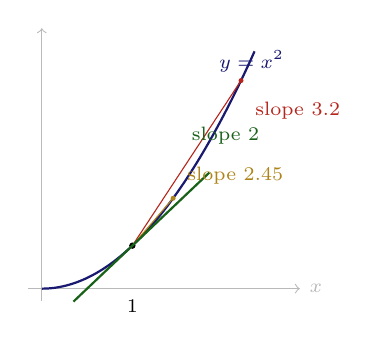
\begin{tikzpicture}[x=1.15cm,y=1.05cm]
  \draw[gray!55,->] (-0.15,0) -- (2.85,0) node[right,font=\scriptsize] {$x$};
  \draw[gray!55,->] (0,-0.15) -- (0,3.15);
  \draw[MidnightBlue,thick] plot[smooth,domain=0:2.35,samples=40] (\x,{0.52*\x*\x});
  \fill (1,0.52) circle (1.15pt);
  \draw[BrickRed] (1,0.52) -- (2.2,{0.52*2.2*2.2});
  \fill[BrickRed] (2.2,{0.52*2.2*2.2}) circle (0.9pt);
  \draw[Goldenrod!80!black] (1,0.52) -- (1.45,{0.52*1.45*1.45});
  \fill[Goldenrod!80!black] (1.45,{0.52*1.45*1.45}) circle (0.9pt);
  % tangent: screen slope is 0.52 * 2 = 1.04
  \draw[ForestGreen!70!black,thick] (0.35,{0.52-1.04*0.65}) -- (1.85,{0.52+1.04*0.85});
  \node[font=\scriptsize,anchor=west,MidnightBlue] at (1.85,2.75) {$y=x^2$};
  \node[font=\scriptsize,anchor=west,BrickRed] at (2.25,2.15) {slope $3.2$};
  \node[font=\scriptsize,anchor=south west,Goldenrod!80!black] at (1.5,1.15) {slope $2.45$};
  \node[font=\scriptsize,anchor=west,ForestGreen!70!black] at (1.55,1.85) {slope $2$};
  \node[font=\scriptsize,anchor=north] at (1,-0.02) {$1$};
\end{tikzpicture}
